%%%%%%%%%%%%%%%%%%%%%%%%%%%%%%%%%%%%%%%%%%%%%%%%%%%%%%
%%%%%%%%%%%%%%%%%%%%%%%%%%%%%%%%%%%%%%%%%%%%%%%%%%%%%%
%%%%%%%%%%%%%%%%%%%%%%%%%%%%%%%%%%%%%%%%%%%%%%%%%%%%%%
\subsection{Standard Model like toys}

\begin{figure}[h]
\centering
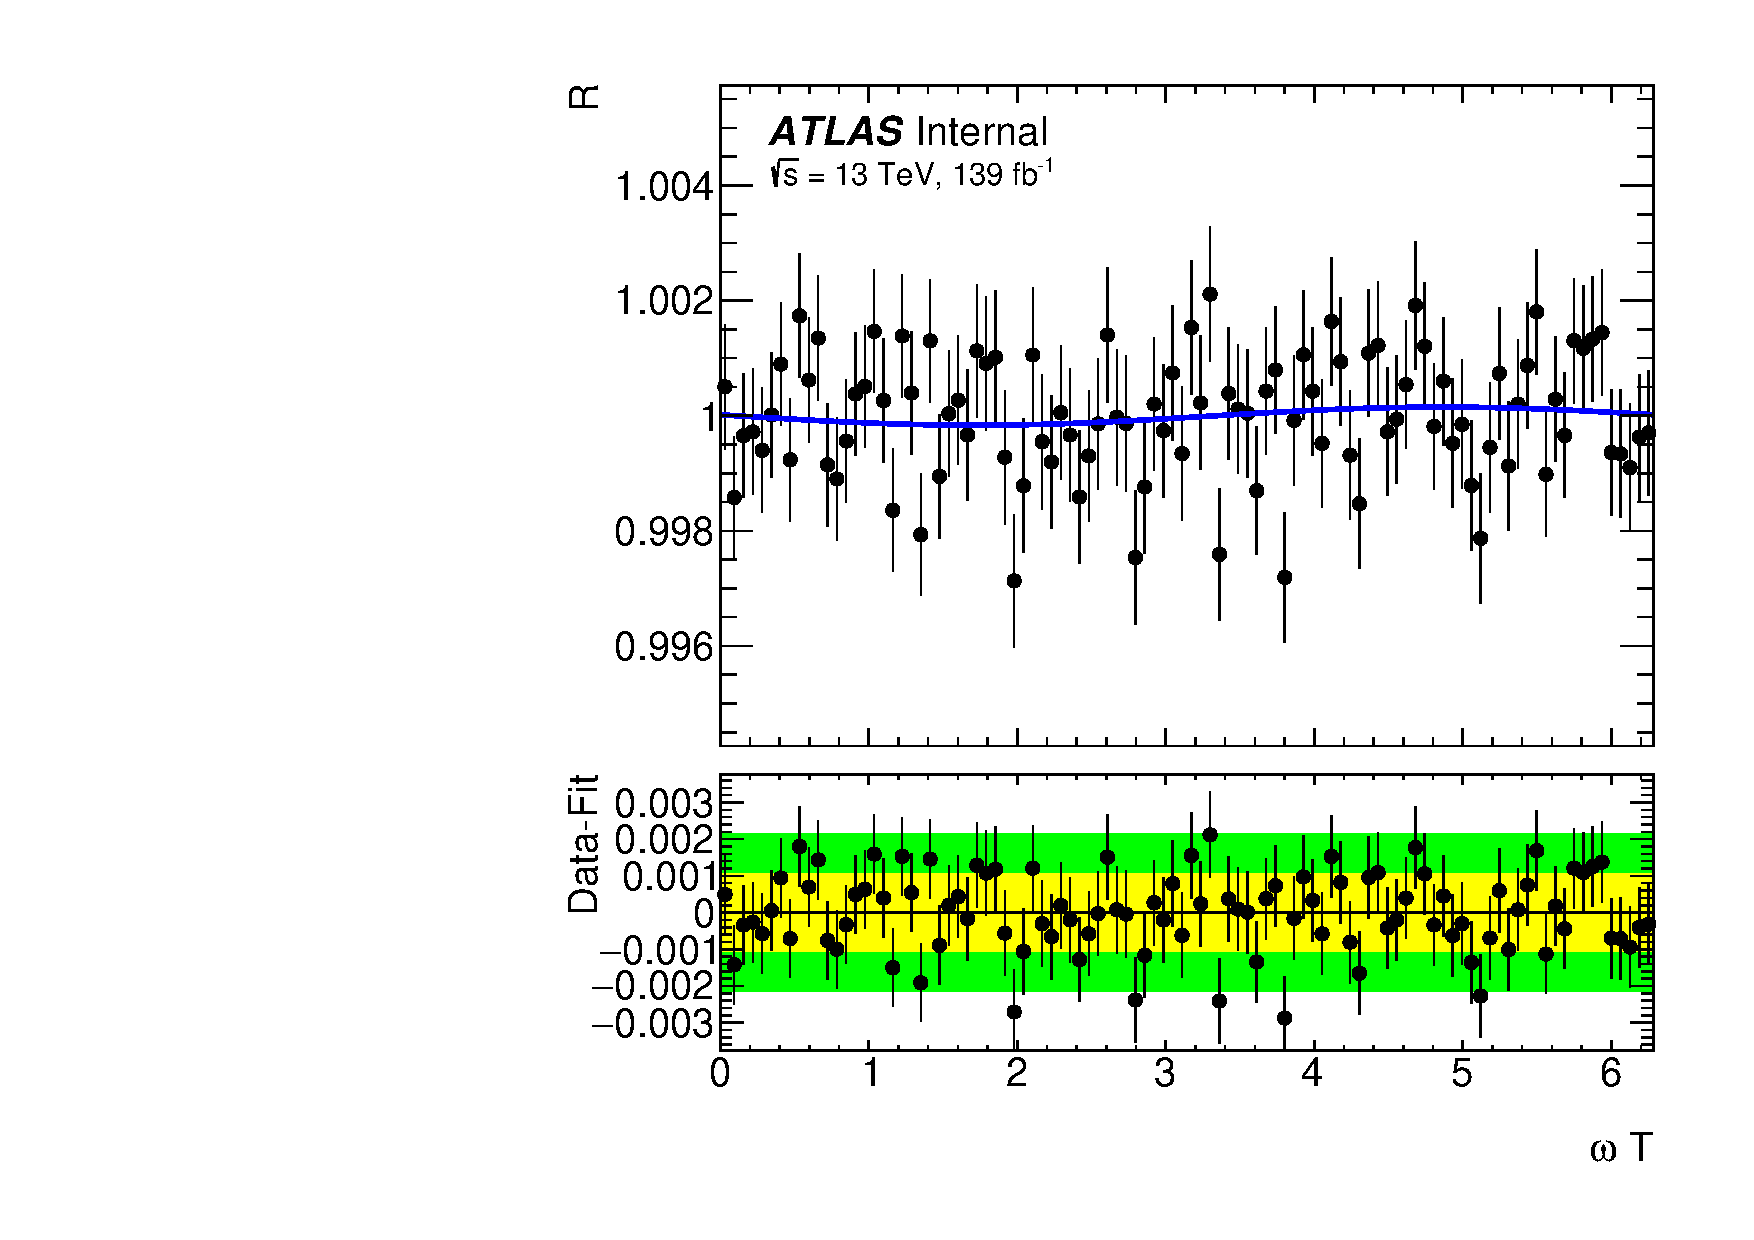
\includegraphics[width=0.45\textwidth]{figs/scrambling/fit_results_d[u,X,Z]_101_residual_12func_SM}
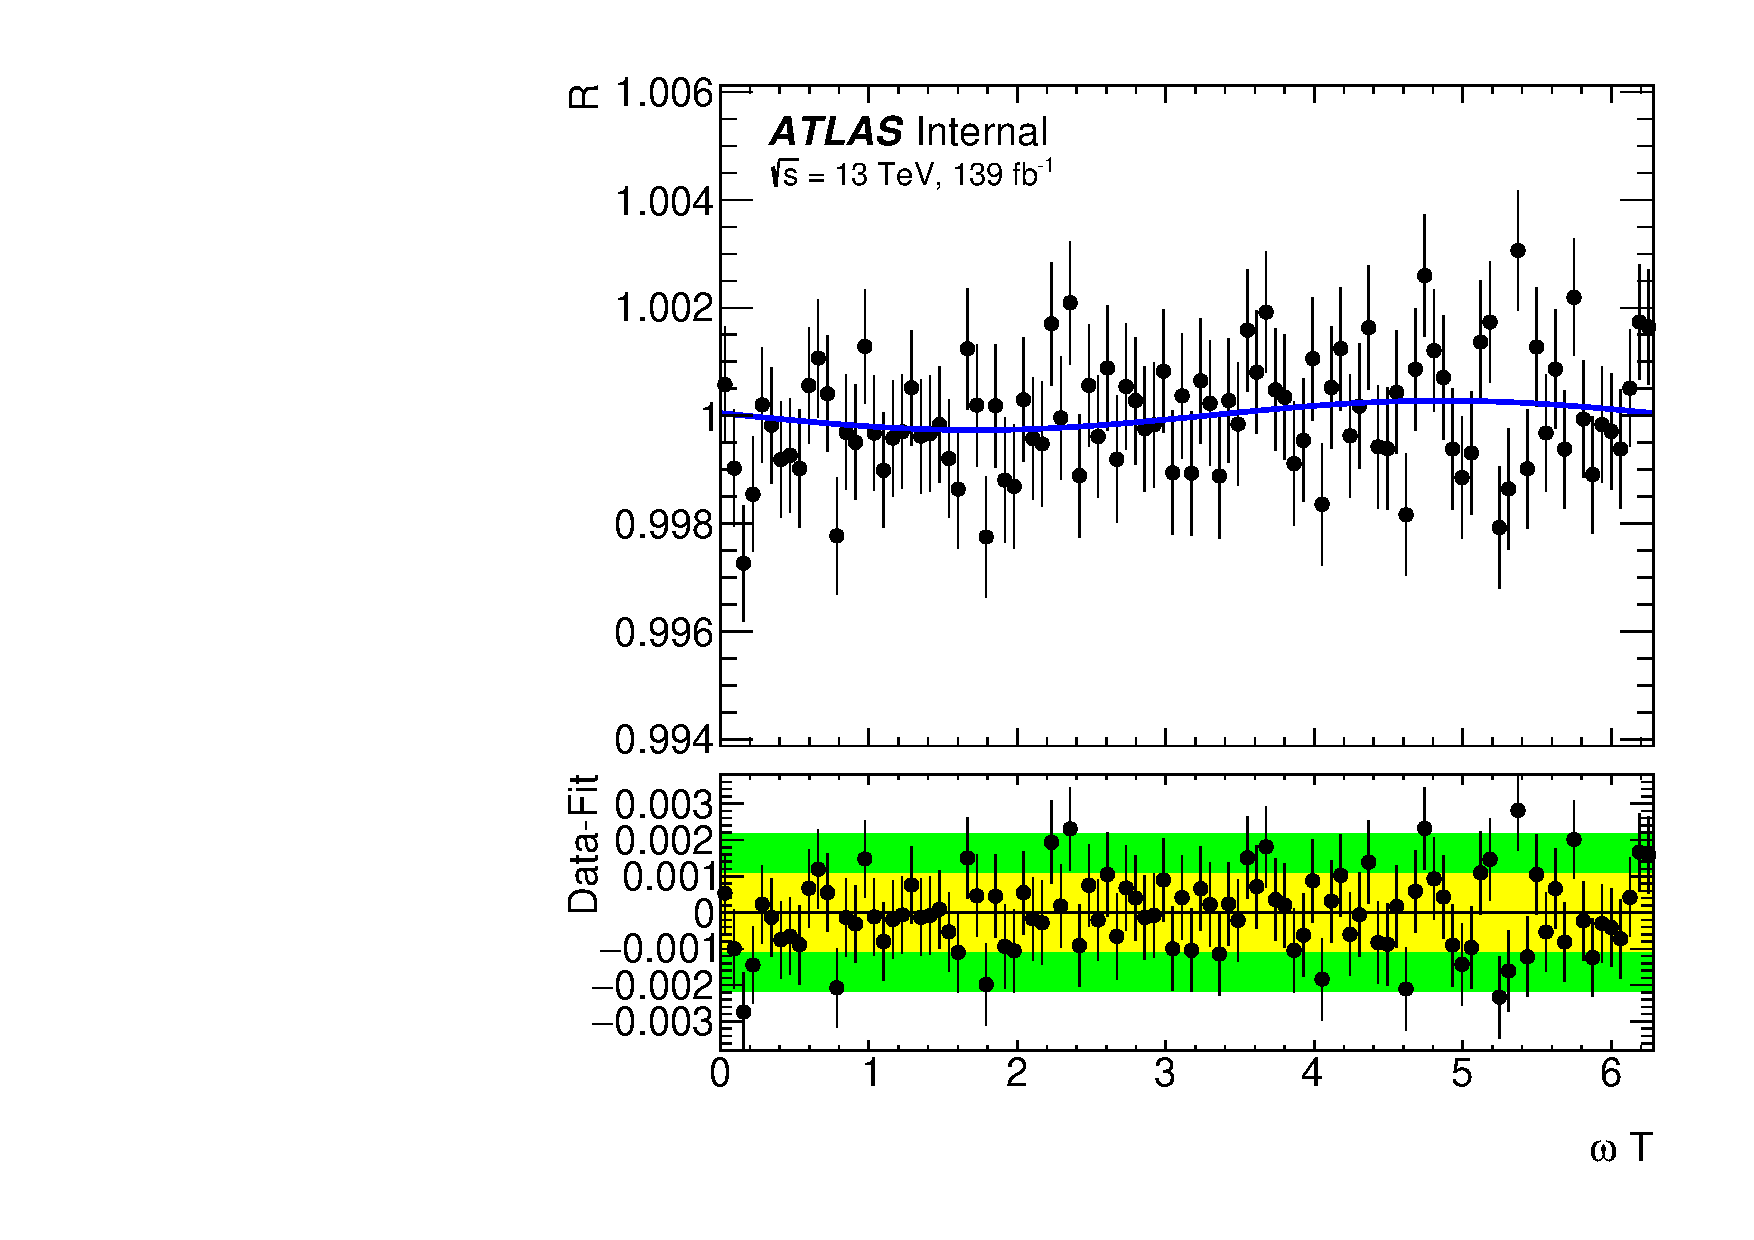
\includegraphics[width=0.45\textwidth]{figs/scrambling/fit_results_d[u,X,Z]_101_residual_12func_SM_scrampled}
\caption{SM-like toy dataset (left), which corresponds to full Run 2 luminosity, and scrambled SM-like toy dataset (right). SM-like toys are signal-free datsets ($\sigma_{LIV}/\sigma_{SM} = 0$). The X-axis is the sidereal phase, $\omega T$. The blue line corresponds to the $d_{u}^{X,Z}$ signal shape after fit to the toy dataset. Bottom panel in each plot is the residual (data-fit)}
\label{fig:SM_like_toy_scrambled}
\end{figure}



\begin{figure}[h]
\centering
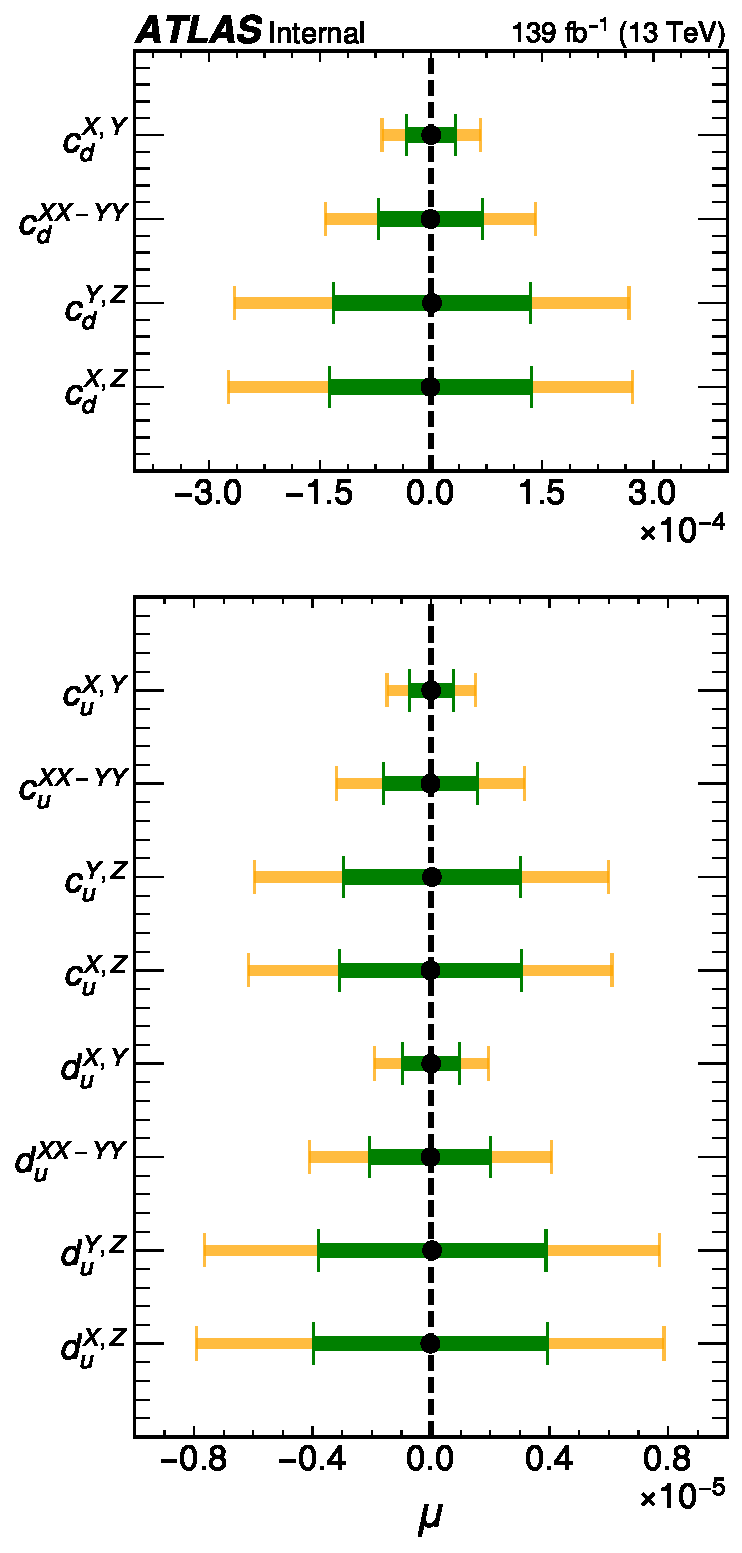
\includegraphics[width=0.45\textwidth]{figs/scrambling/SigFit_summary_AllSamples_SM}
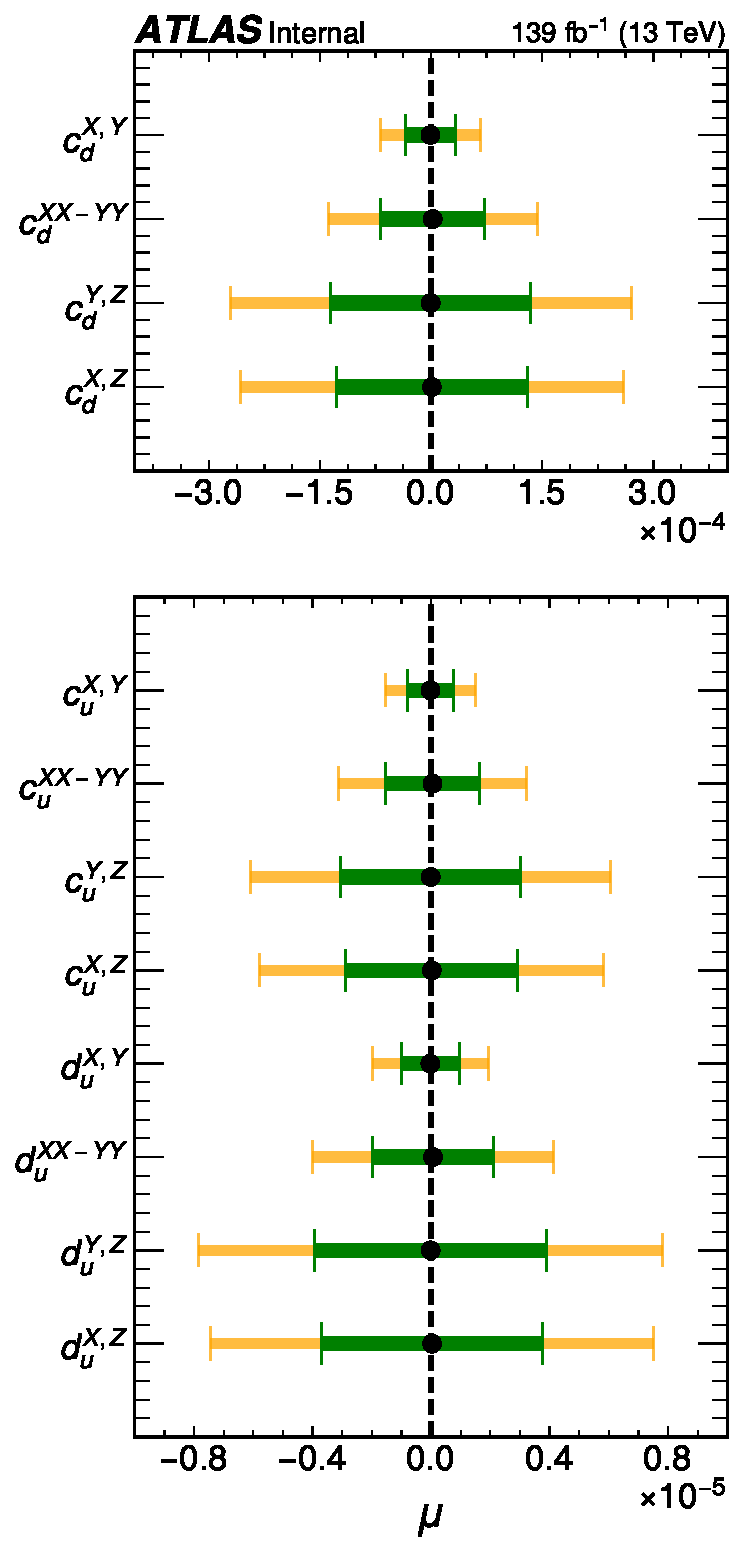
\includegraphics[width=0.45\textwidth]{figs/scrambling/SigFit_summary_AllSamples_SM_scrambled}
\caption{Fit results obtained from 1000 SM-like toy datasets. Results on SM-like toy datasets (left), which corresponds to full Run 2 luminosity, and scrambled SM-like toy datasets (right). SM-like toys are signal-free datsets ($\sigma_{LIV}/\sigma_{SM} = 0$). Y-axis corresponds to 12 exact signal shapes from SME. The X-axis is the signal strength. Yellow and green bends correspond to one and two signal uncertainty bands. }
\label{fig:SM_like_toy_fit_results12}
\end{figure}

%%%%%%%%%%%%%%%%%%%%%%%%%%%%%%%%%%%%%%%%%%%%%%%%%%%%%%
%%%%%%%%%%%%%%%%%%%%%%%%%%%%%%%%%%%%%%%%%%%%%%%%%%%%%%
%%%%%%%%%%%%%%%%%%%%%%%%%%%%%%%%%%%%%%%%%%%%%%%%%%%%%%
\subsection{Signal injected toys}

\begin{figure}[h]
\centering
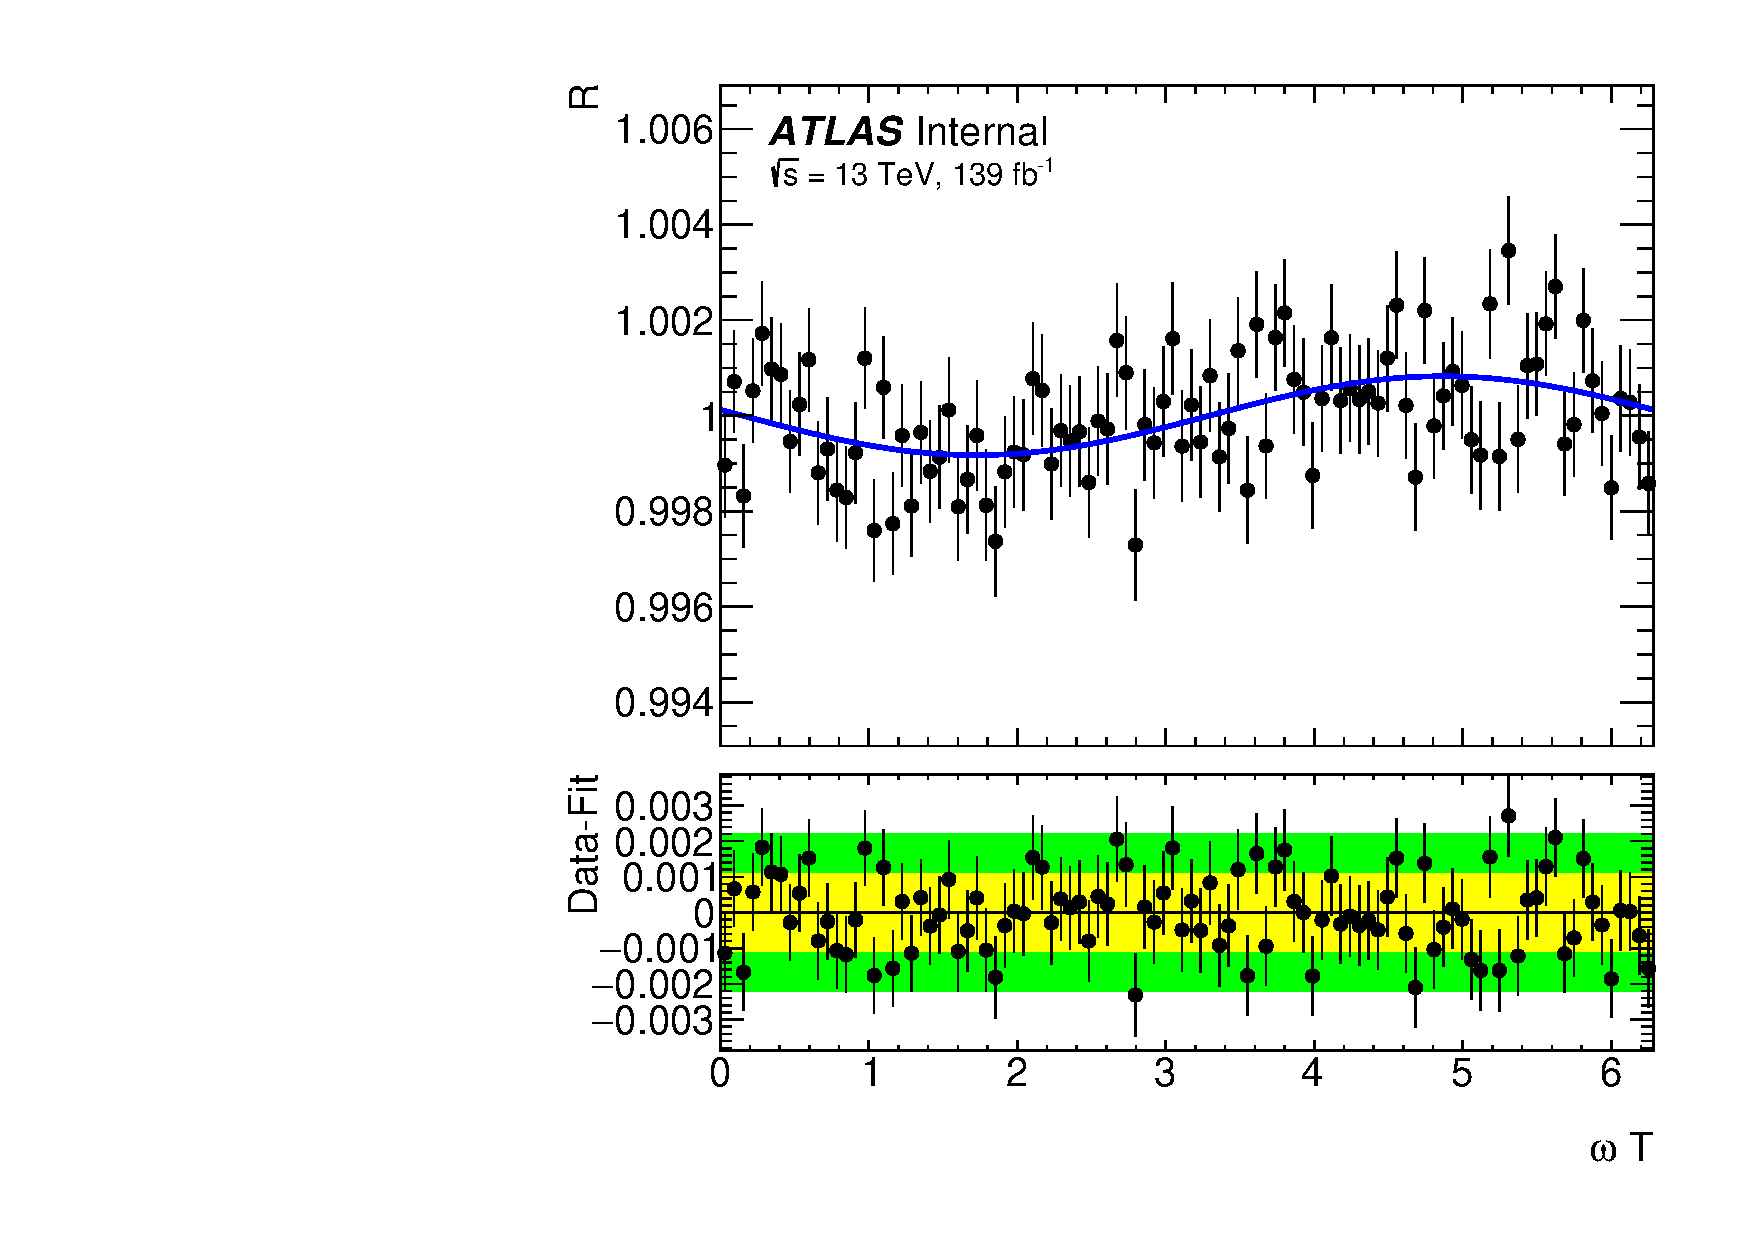
\includegraphics[width=0.45\textwidth]{figs/scrambling/fit_results_d[u,X,Z]_101_residual_12func_sigP0015}
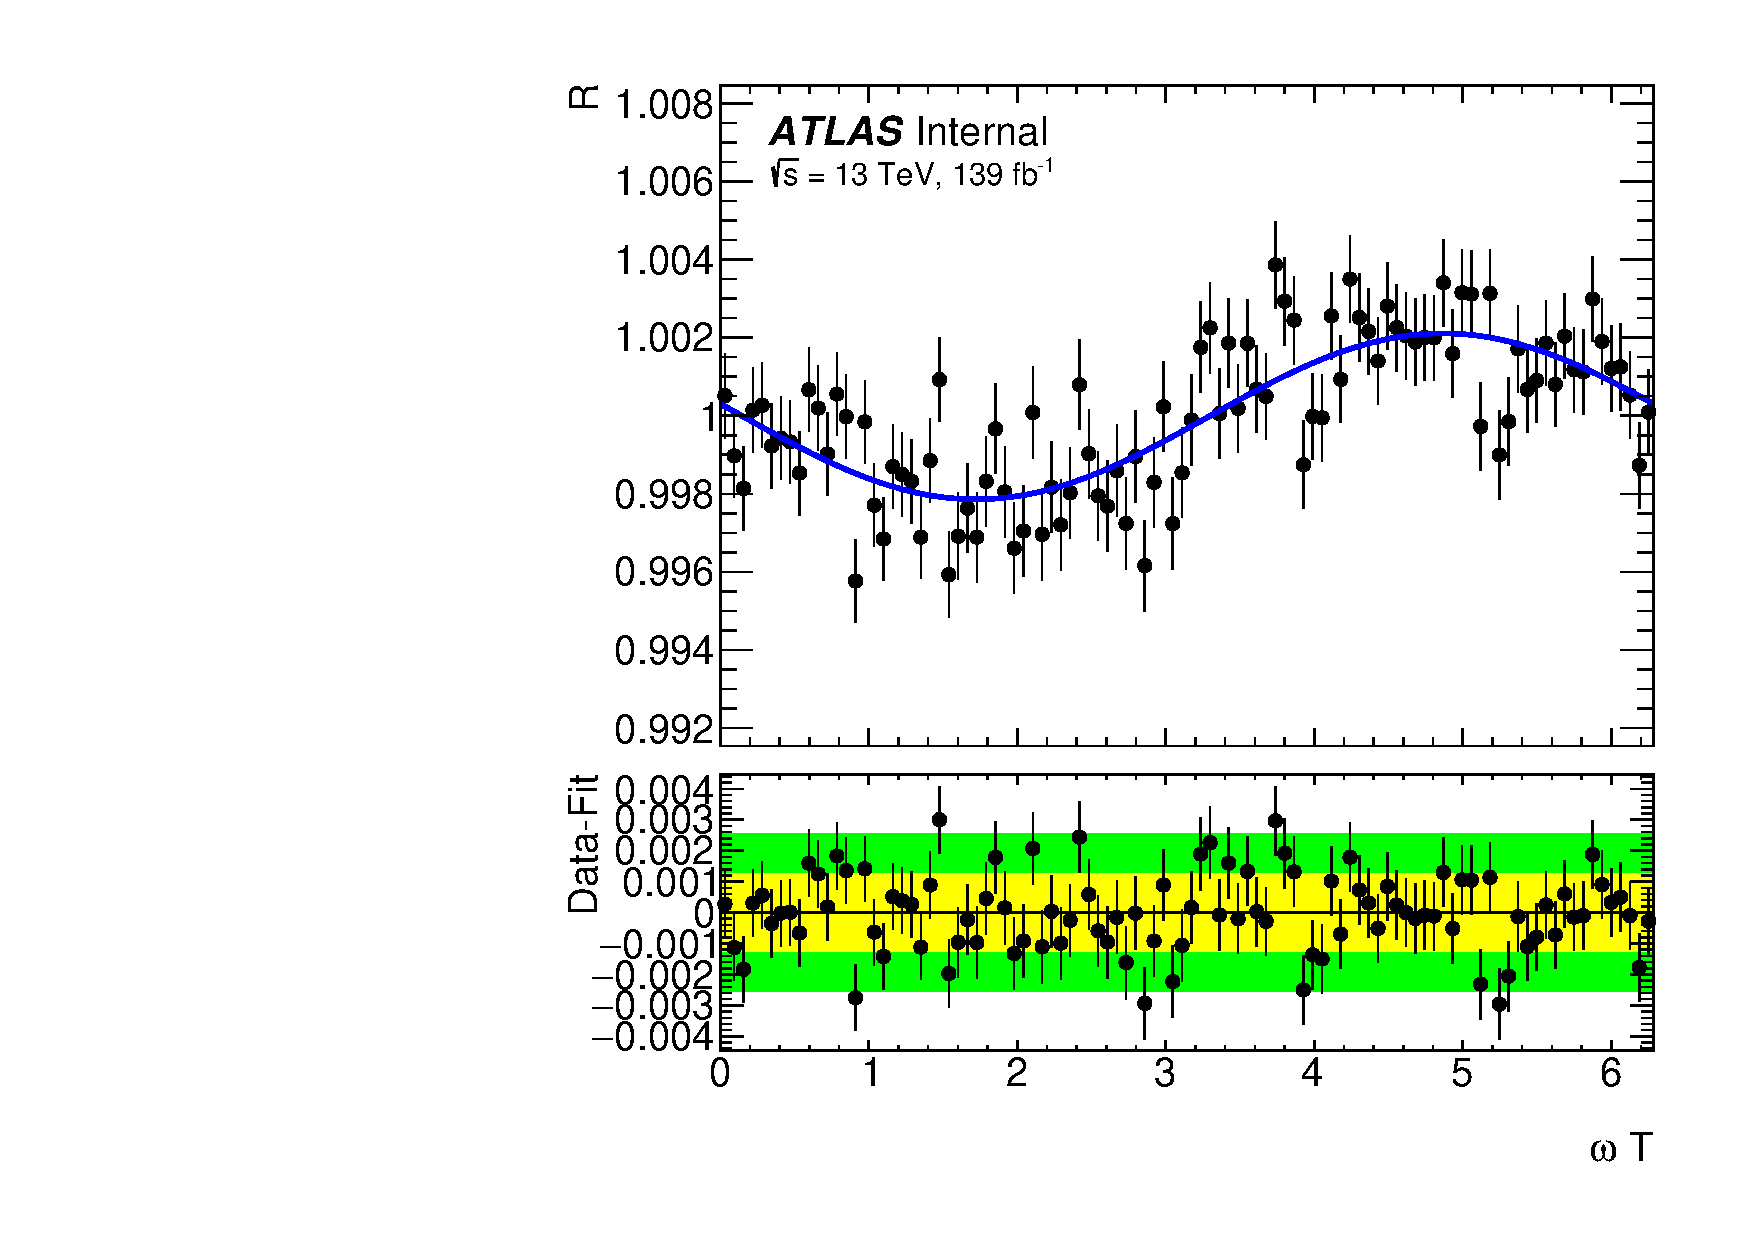
\includegraphics[width=0.45\textwidth]{figs/scrambling/fit_results_d[u,X,Z]_101_residual_12func_sigP003}
\caption{A signal injected toy dataset. The injected signal shape is $d_{u}^{X,Z}$ from SME. The njected signal fractions ($\sigma_{LIV}/\sigma_{SM}$)  are 0.0015 (left) and 0.003 (right). The blue line is the signal ($d_{u}^{X,Z}$) after fit to the toy dataset. Bottom panel in each plot is the residual (data-fit). The X-axis is the sidereal phase, $\omega  T$.}
\label{fig:signal_injected_toy_p003_p0015}
\end{figure}




\begin{figure}[h]
\centering
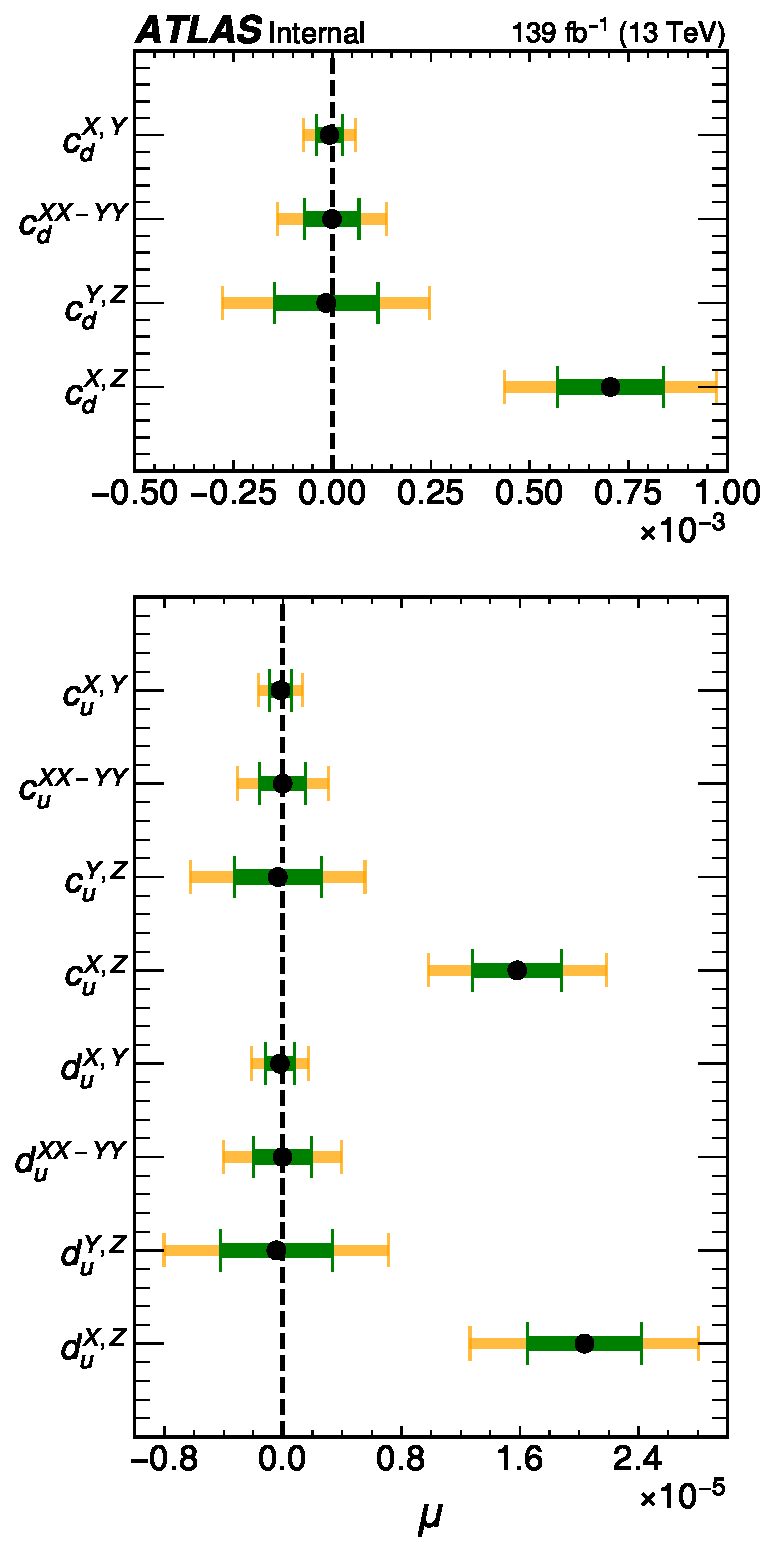
\includegraphics[width=0.45\textwidth]{figs/scrambling/SigFit_summary_AllSamples_sigP0015}
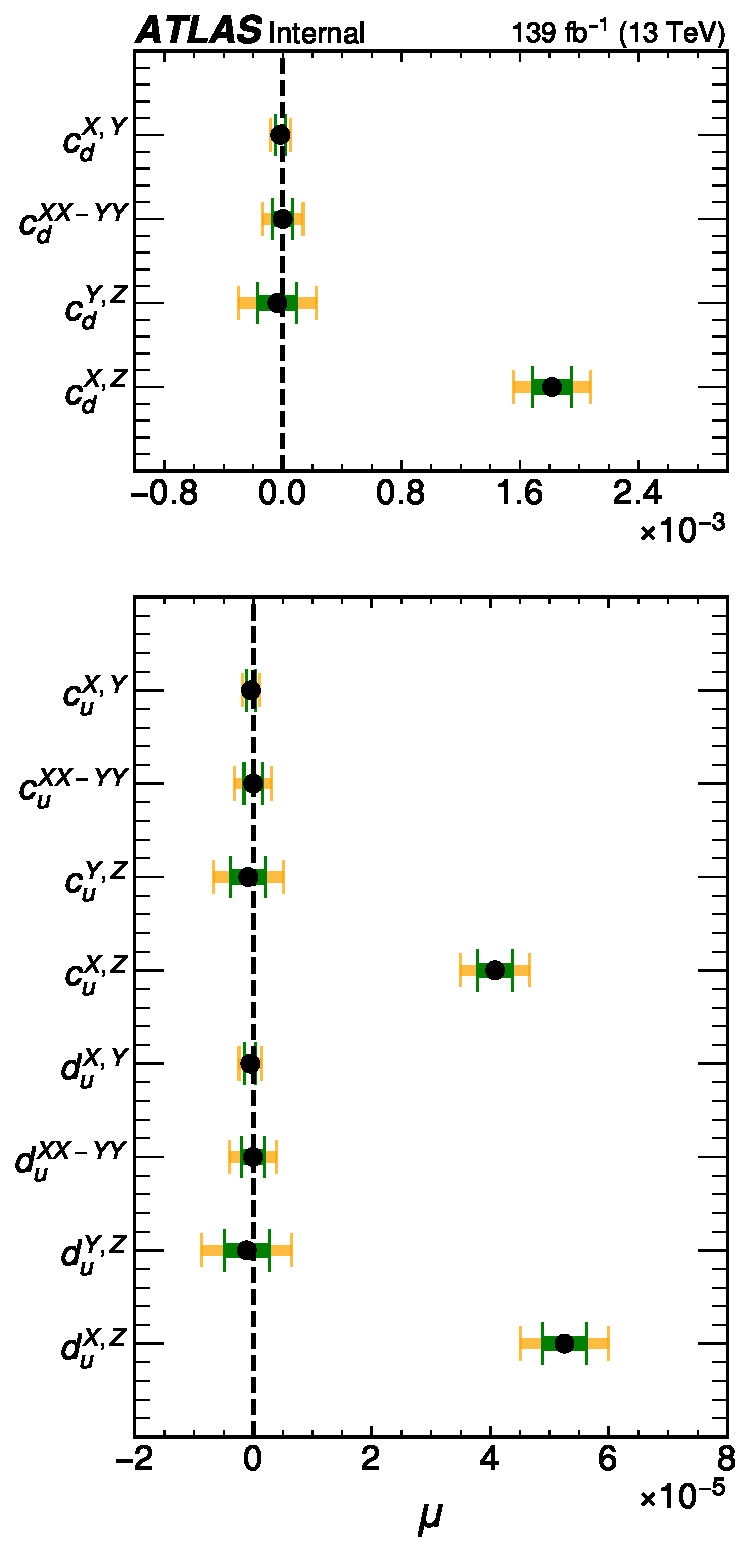
\includegraphics[width=0.44\textwidth]{figs/scrambling/SigFit_summary_AllSamples_sigP003}
\caption{Fit results from 1000 signal injected toys. The injected signal shape is $d_{u}^{X,Z}$ from SME. The njected signal fractions ($\sigma_{LIV}/\sigma_{SM}$)  are 0.0015 (left) and 0.003 (right). Y-axis corresponds to 12 exact signal shapes from SME. The X-axis is the signal strength.}
\label{fig:signal_injected_toy_p003_p0015_fit_results12}
\end{figure}






\begin{figure}[h]
\centering
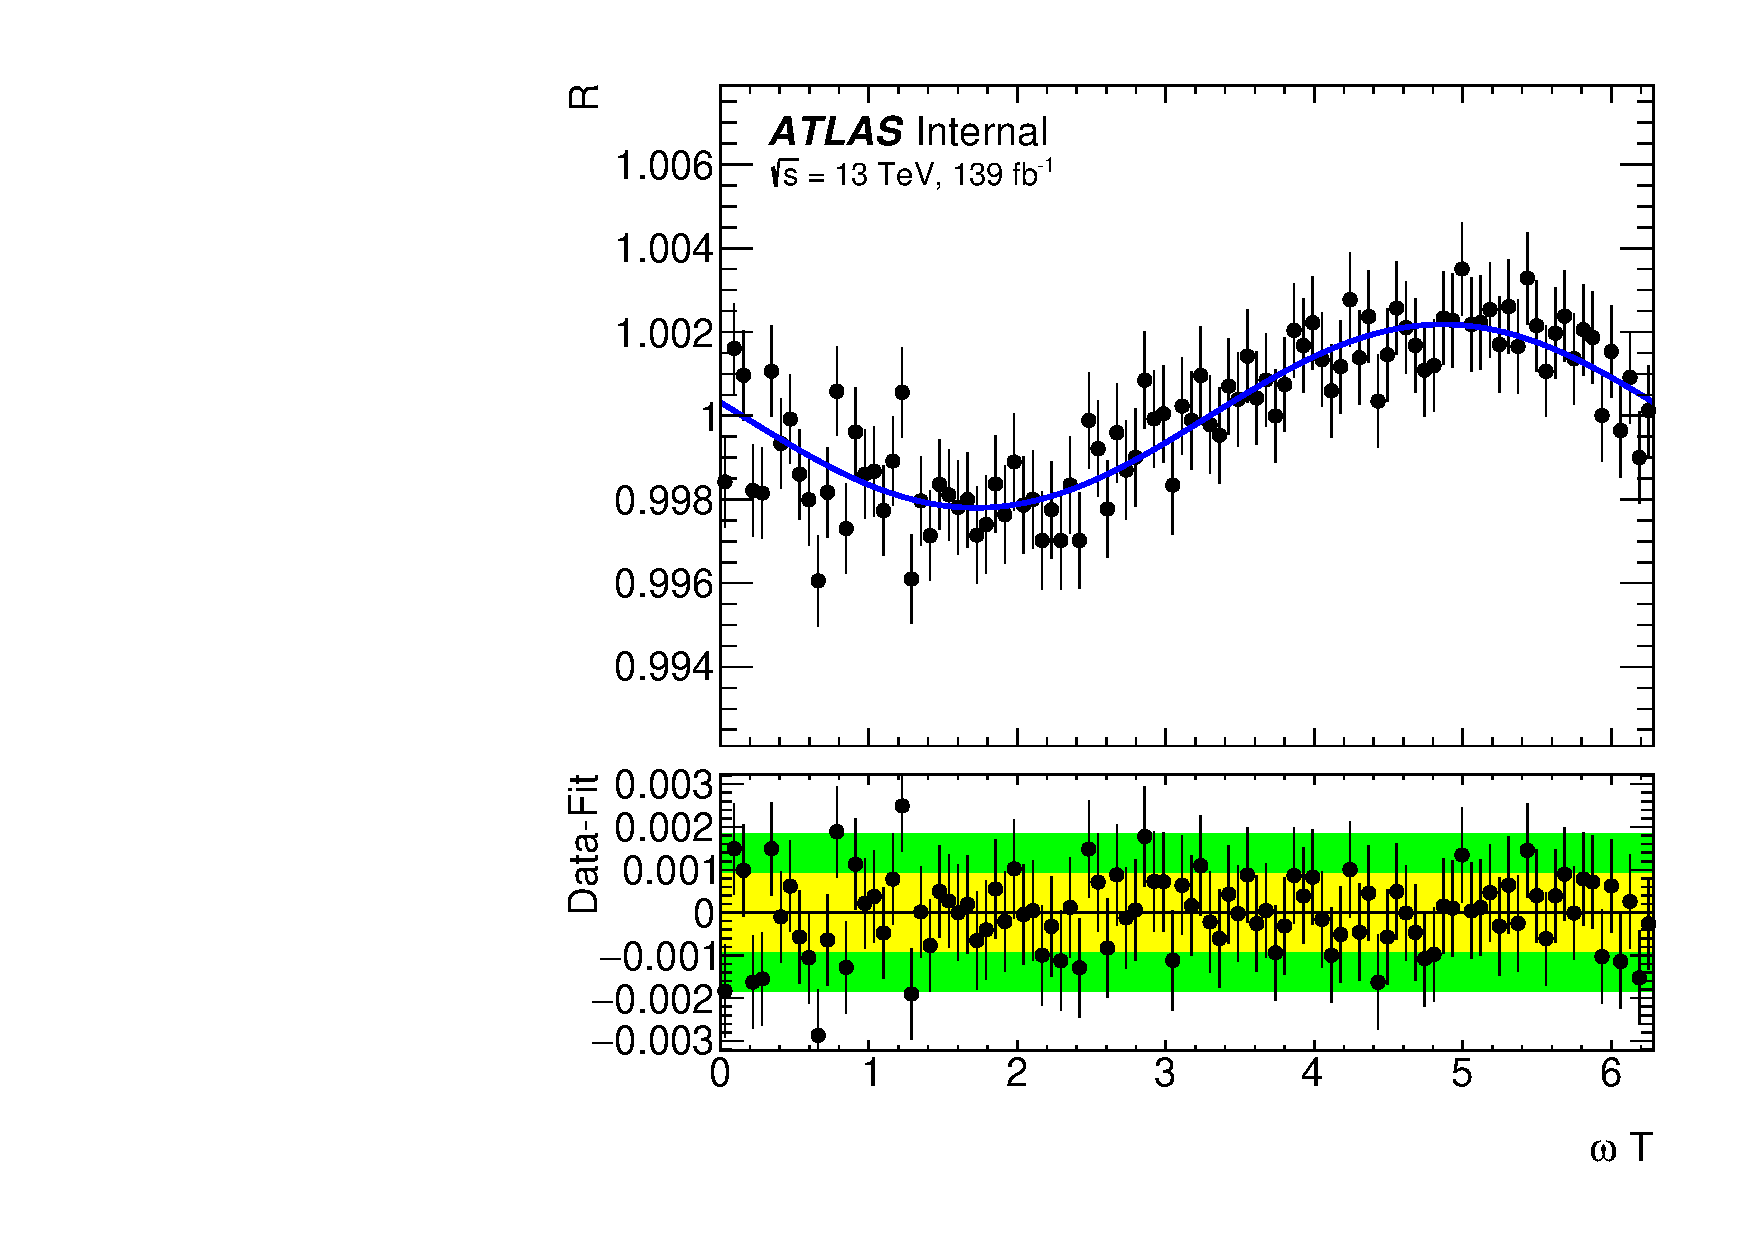
\includegraphics[width=0.45\textwidth]{figs/scrambling/fit_results_d[u,X,Z]_5170_residual_12func_sigP003}
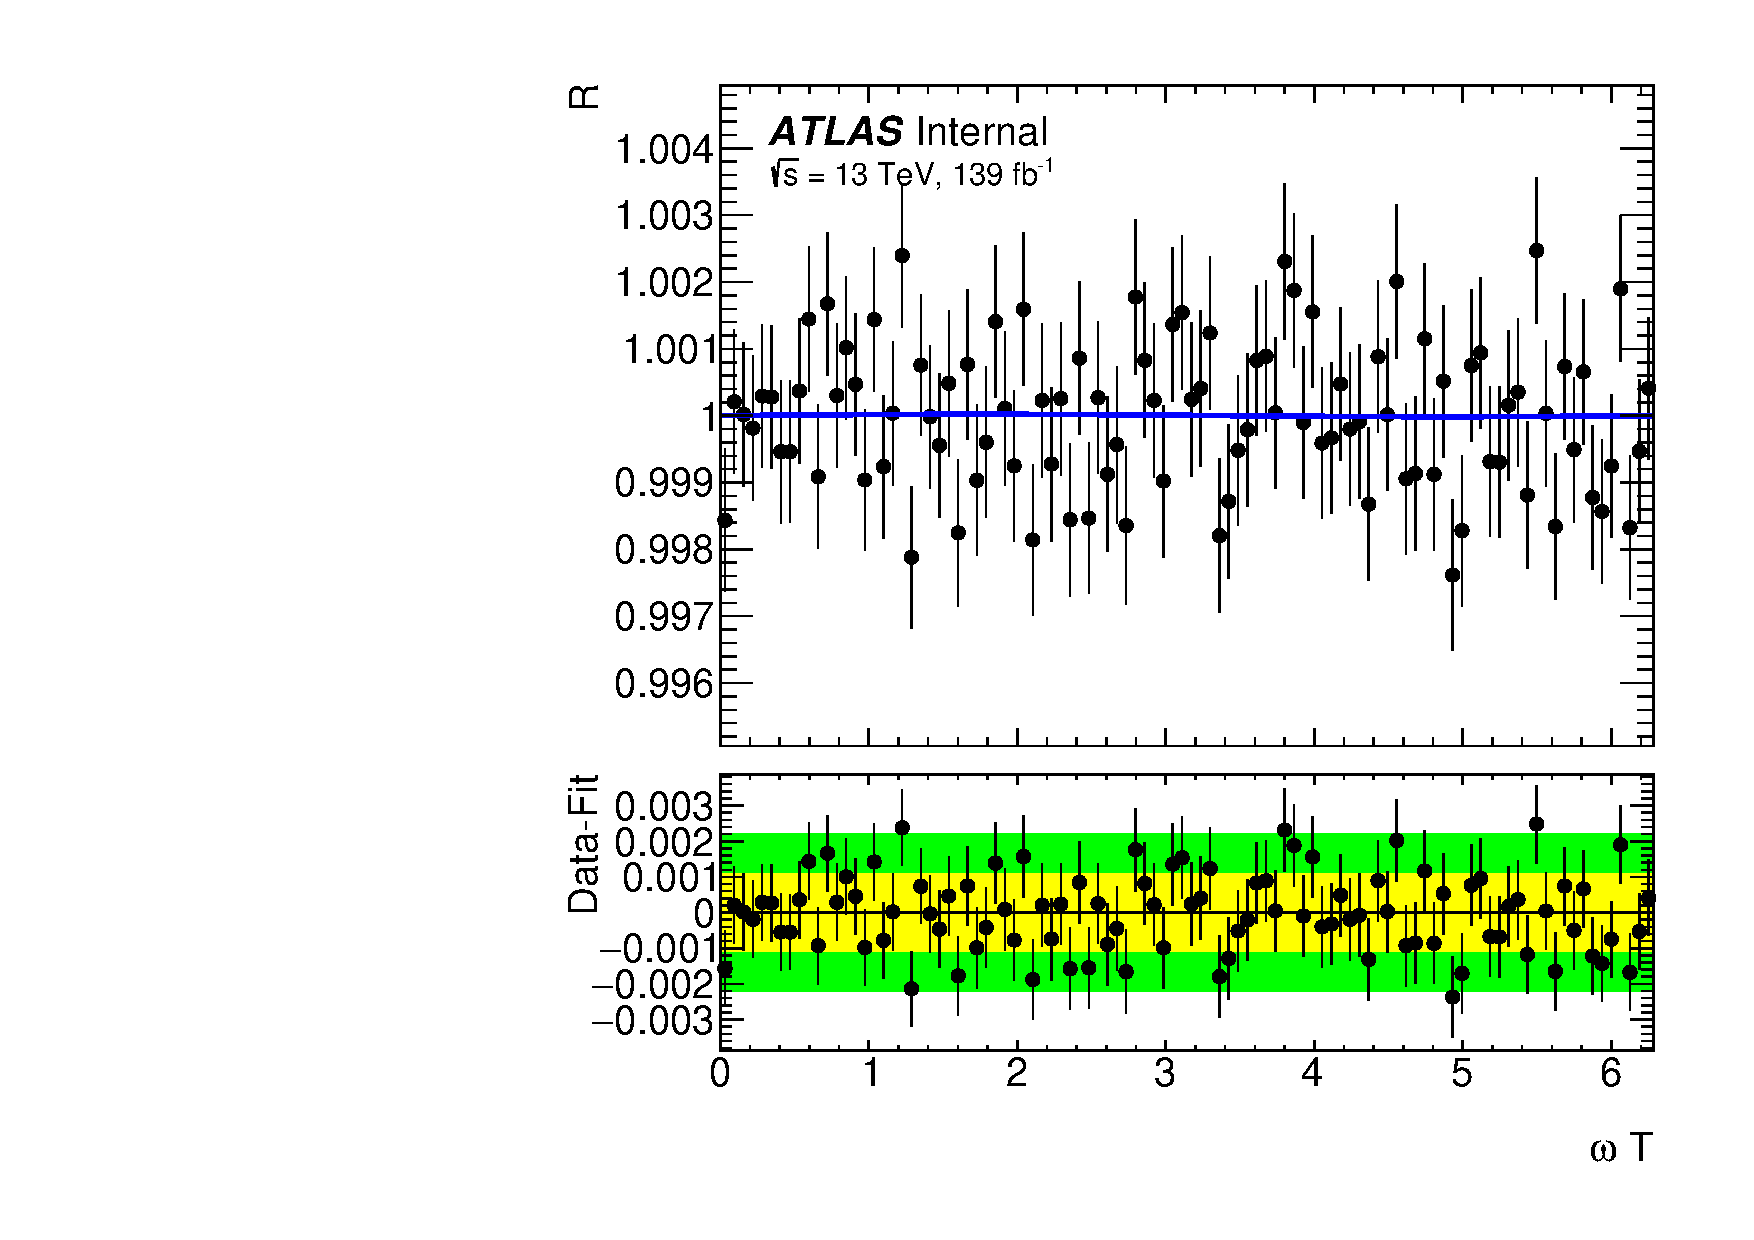
\includegraphics[width=0.45\textwidth]{figs/scrambling/fit_results_c[d,X,Z]_5170_residual_12func_sigP003_scrambled}
    \caption{Comparison of a signal injected toy dataset before and after a scramble. The injected signal shape is $d_{u}^{X,Z}$ from SME. The injected signal fractions ($\sigma_{LIV}/\sigma_{SM}$)  is 0.003. The original toy dataset (left) and scrambled data (right). The blue line is the signal ($d_{u}^{X,Z}$) after fit to the toy dataset. The bottom panel in each plot is the residual (data - fit). The X-axis is the sidereal phase, $\omega T$.
The Fitted signal strength is $5.3E^{-5}\pm 3.8E^{-6}$ (left), and $-4.4E^{-7}\pm 3.8E^{-6}$ (right) after scrambling. 
}
\label{fig:signal_injected_toy_p003_beforeAfter_scramble}
\end{figure}
